\chapter{Conclusion - Chapter is Work In Progress}
It is time to look back at the work that has been done, to highlight the progress that has been made, but also the shortcomings and gaps that need to be filled by future improvements. We will therefore use this chapter to discuss some of the key points that emerge from this thesis.
 
\section{Intended use of the FuxCP tool}
Throughout this work, it is clear that all the examples provided are fairly short (fourteen bars at most). This is primarily due to Fux himself, as the examples he gives are always of the same shortness, probably for pedagogical purposes. He does not mention this explicitly, but there may also be a practical reason for considering only such short compositions. Indeed, these small compositions can be considered as 'blocks', which can then be arranged to form a whole. The great advantage of this approach is that the countrepoints can be given different species between the blocks, allowing the composition to be constantly renewed.

\begin{figure}[h]
  \centering
  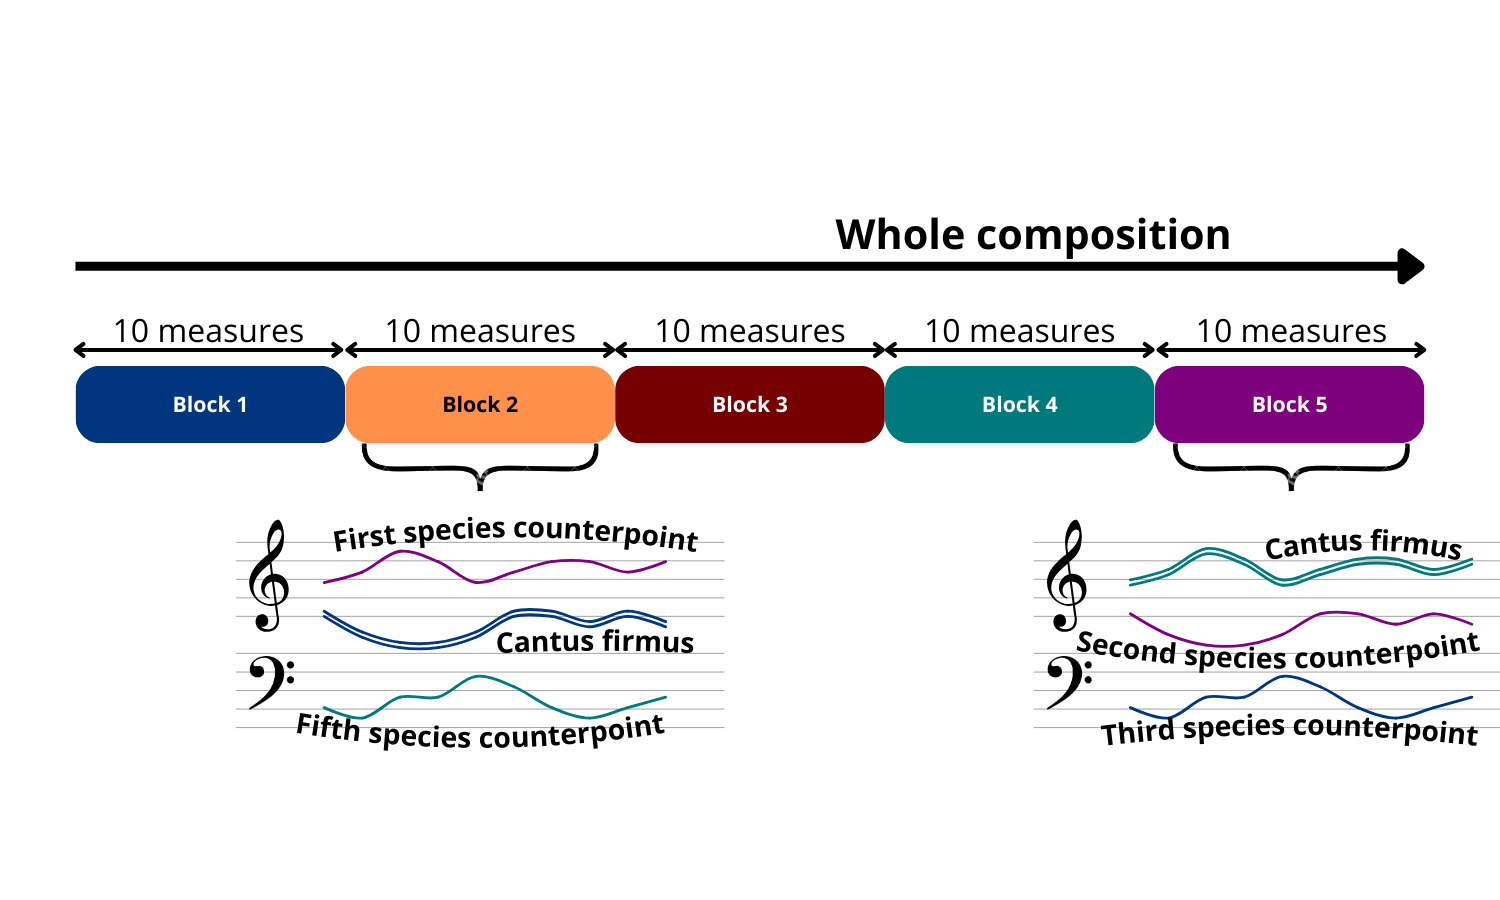
\includegraphics[width=1\textwidth]{Images/composition-in-blocks.png}
  \caption{Example of what of a composition in blocks could look like}
  \label{fig:composition-in-blocks}
\end{figure}

\section{Known issues about the current state of the work}
\begin{itemize}
  \item As mentioned in section \ref{section:time-to-find-a-solution}, some few combinations of species, voice ranges and \textit{cantus firmi} cause the solver to fail to find a solution. The current roundabout way to "solve" this is to... change the voice ranges or some other parameter until a structural solution is found. These cases are relatively rare and do not prevent the use of FuxCP.
  \item If a counterpoint of the fourth species is the lowest stratum, the solver needs more time to find a solution in which all notes are ligated. This is not a problem when combining a fourth species counterpoint with a simple species counterpoint (first or second species), but becomes difficult to handle with more complex species (third or fifth species), as the search time before the solver finds a suitable solution (i.e. with all notes tied) can become very long.
\end{itemize}




